% Standalone XeLaTeX source. Source: 2024ap_exam.pdf, PDF p. 2 (exam 2024-08-27).
\documentclass[10pt,a4paper]{article}
\usepackage[margin=20mm]{geometry}
\usepackage{fontspec}
\usepackage{xeCJK}
\setCJKmainfont{HaranoAjiMincho-Regular.otf}
\setCJKsansfont{HaranoAjiGothic-Medium.otf}
\usepackage{amsmath,amssymb}
\usepackage{tikz}
\usepackage{caption}
\setlength{\parindent}{1em}
\setlength{\parskip}{0.24em}
\title{物理工学専攻 院試解答集 ver2\\2024年 物理学 第1問}
\author{政岡凜太郎}
\date{}
\begin{document}
\maketitle

質点の質量を$m$、自然角周波数を$\omega_0$、粘性抵抗係数を$\zeta$とする。バネによる復元力は $-m\omega_0^2x$ であるから、両部分で用いる運動方程式は
\begin{equation}
 m\ddot x(t)+\zeta\dot x(t)+m\omega_0^2x(t)=f(t).
 \label{eq:motion}
\end{equation}
位置の正方向は自然長の位置を原点とする $x$ 軸の正方向とする。

\section*{[1.1] 周期外力に対する定常解}
この節では周期外力$f(t)=F_0e^{i\Omega t}$（$\Omega>0$）を加える。外力と同じ時間因子をもつ定常解 $x(t)=X_0e^{i\Omega t}$ を式\eqref{eq:motion}に代入する。$\dot x=i\Omega x$、$\ddot x=-\Omega^2x$ なので
\[
\{m(\omega_0^2-\Omega^2)+i\zeta\Omega\}X_0=F_0.
\]
$\zeta>0$ かつ $\Omega>0$ で分母はゼロにならない。したがって、過渡項が減衰した後の複素表示は
\begin{equation}
\boxed{x(t)=\frac{F_0e^{i\Omega t}}{m(\omega_0^2-\Omega^2)+i\zeta\Omega}}.
\label{eq:steady}
\end{equation}
実際の位置が必要なら、この複素式の実部を取る。

\section*{[1.2] 応答関数の実部と虚部}
式\eqref{eq:steady}を $f(t)=F_0e^{i\Omega t}$ で割り、分母の共役複素数を掛ける。$D(\Omega)=m^2(\omega_0^2-\Omega^2)^2+\zeta^2\Omega^2>0$ とおくと
\begin{equation}
\varepsilon=\frac{m(\omega_0^2-\Omega^2)-i\zeta\Omega}{D(\Omega)},\qquad
\boxed{\varepsilon'=\frac{m(\omega_0^2-\Omega^2)}{D(\Omega)},\quad
\varepsilon''=-\frac{\zeta\Omega}{D(\Omega)}}.
\label{eq:response}
\end{equation}
$e^{i\Omega t}$ を選んだため減衰項は分母で $+i\zeta\Omega$ となり、$\Omega>0$ で $\varepsilon''<0$ である。固有角周波数 $\Omega=\omega_0$ では $\varepsilon'=0$、$-\varepsilon''=1/(\zeta\omega_0)$ となる。

\section*{[1.3] 弱減衰・近共鳴での概形と極値}
$\Delta=\Omega-\omega_0$、$\gamma=\zeta/(2m)$ とおく。弱減衰$\gamma\ll\omega_0$かつ$|\Delta|\ll\omega_0$ の範囲では $\omega_0^2-\Omega^2\simeq-2\omega_0\Delta$、$\zeta\Omega\simeq\zeta\omega_0$ だから
\begin{equation}
\varepsilon'\simeq-\frac{\Delta}{2m\omega_0(\Delta^2+\gamma^2)},\qquad
-\varepsilon''\simeq\frac{\gamma}{2m\omega_0(\Delta^2+\gamma^2)}.
\label{eq:near}
\end{equation}
第一式を $\Delta$ で微分すると極値条件は $\Delta^2=\gamma^2$ である。よって $\varepsilon'$ の正の極大は $\Omega\simeq\omega_0-\gamma$、負の極小は $\Omega\simeq\omega_0+\gamma$ にある。第二式は $\Delta=0$ で極大となる。下図は横軸を $\Delta/\gamma$ とする近共鳴領域の概形であり、縦軸は両関数に共通の $A=1/(2m\omega_0\gamma)$ で割っている。

\begin{figure}[htbp]
\centering
\begin{minipage}{0.48\linewidth}\centering
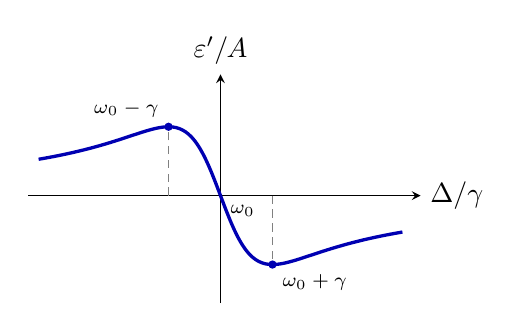
\begin{tikzpicture}[x=0.66cm,y=1.75cm,>=stealth]
 \draw[->] (-3.7,0)--(3.85,0) node[right] {$\Delta/\gamma$};
 \draw[->] (0,-0.78)--(0,0.88) node[above] {$\varepsilon'/A$};
 \draw[blue!70!black,very thick,smooth,samples=120,domain=-3.5:3.5] plot (\x,{-\x/(1+\x*\x)});
 \draw[densely dashed,gray] (-1,0)--(-1,0.5);
 \draw[densely dashed,gray] (1,0)--(1,-0.5);
 \fill[blue!70!black] (-1,0.5) circle (1.5pt);
 \fill[blue!70!black] (1,-0.5) circle (1.5pt);
 \node[above left,font=\scriptsize] at (-1,0.5) {$\omega_0-\gamma$};
 \node[below right,font=\scriptsize] at (1,-0.5) {$\omega_0+\gamma$};
 \node[below right,font=\scriptsize] at (0,0) {$\omega_0$};
\end{tikzpicture}
\end{minipage}\hfill
\begin{minipage}{0.48\linewidth}\centering
\begin{tikzpicture}[x=0.66cm,y=1.45cm,>=stealth]
 \draw[->] (-3.7,0)--(3.85,0) node[right] {$\Delta/\gamma$};
 \draw[->] (0,-0.12)--(0,1.35) node[above] {$-\varepsilon''/A$};
 \draw[red!70!black,very thick,smooth,samples=120,domain=-3.5:3.5] plot (\x,{1/(1+\x*\x)});
 \fill[red!70!black] (0,1) circle (1.5pt);
 \node[above right,font=\scriptsize] at (0,1) {極大 $\Omega\simeq\omega_0$};
 \node[below right,font=\scriptsize] at (0,0) {$\omega_0$};
\end{tikzpicture}
\end{minipage}
\caption{近共鳴の $\varepsilon'$ と $-\varepsilon''$。左右の横軸の原点は $\Omega=\omega_0$ に対応する。}
\label{fig:resonance}
\end{figure}

\section*{[2.1] 平均二乗変位}
ここから $x,f$ は実数であり、角括弧は定常状態のアンサンブル平均を表す。問題で与えられた平均零$\langle f\rangle=0$と同時刻の$x(t),f(t)$の無相関を用いる。式\eqref{eq:motion}に $x(t)$ を掛けて平均すると
\[
 m\langle x\ddot x\rangle+\zeta\langle x\dot x\rangle+m\omega_0^2\langle x^2\rangle=\langle xf\rangle=\langle x\rangle\langle f\rangle=0.
\]
定常状態では $d\langle x^2\rangle/dt=0$ より $\langle x\dot x\rangle=0$。また $d\langle x\dot x\rangle/dt=\langle\dot x^2+x\ddot x\rangle=0$ より $\langle x\ddot x\rangle=-\langle\dot x^2\rangle=-\overline{v^2}$とする。ここで$v=\dot x$、$\overline{v^2}$はその二乗の定常平均である。したがって
\begin{equation}
\boxed{\langle x(t)^2\rangle=\frac{\overline{v^2}}{\omega_0^2}}.
\label{eq:x2}
\end{equation}

\section*{[2.2] フーリエ変換とパワースペクトル}
原本の無限時間表示 $X(\omega)=\int_{-\infty}^{\infty}x(t)e^{-i\omega t}\,dt$ と $F(\omega)=\int_{-\infty}^{\infty}f(t)e^{-i\omega t}\,dt$ を形式的に用いると、時間微分のフーリエ変換は $i\omega X$、二階微分は $-\omega^2X$ となる。定常雑音のスペクトルは、長さ $T>0$ の観測窓で
$X_T(\omega)=\int_{-T/2}^{T/2}x(t)e^{-i\omega t}\,dt$ と
$F_T(\omega)=\int_{-T/2}^{T/2}f(t)e^{-i\omega t}\,dt$ を定め、
$I_x(\omega)=\lim_{T\to\infty}\langle|X_T(\omega)|^2\rangle/T$、
$I_f(\omega)=\lim_{T\to\infty}\langle|F_T(\omega)|^2\rangle/T$ と読む。
有限窓では部分積分により、$D(\omega)=m(\omega_0^2-\omega^2)+i\zeta\omega$ として
\[
 D(\omega)X_T(\omega)=F_T(\omega)
 -\left[e^{-i\omega t}\{m\dot x(t)+(\zeta+i m\omega)x(t)\}\right]_{-T/2}^{T/2}.
\]
定常な $x,\dot x$ の二乗平均が有限なら、角括弧内の端点項の二乗平均は $T$ に依存せず有界である。$\langle|F_T|^2\rangle=O(T)$ のとき、端点項と $F_T$ の交差項も Cauchy--Schwarz の不等式で $O(\sqrt T)$ だから、$T$ で割るスペクトルの極限には寄与しない。したがって、形式的な無限時間の関係と、それが表す定常スペクトルは
\begin{equation}
\boxed{X(\omega)=\frac{F(\omega)}{m(\omega_0^2-\omega^2)+i\zeta\omega}},\qquad
\boxed{I_x(\omega)=\frac{I_f(\omega)}{m^2(\omega_0^2-\omega^2)^2+\zeta^2\omega^2}}.
\label{eq:spectrum}
\end{equation}
後の白色入力では $\langle|F_T|^2\rangle=IT$ となり、上の条件を満たす。


\section*{[2.3] 変位の相関関数}
白色揺動力の相関 $\langle f(t)f(t+\tau)\rangle=I\delta(\tau)$（$I>0$）をフーリエ変換すると、$I_f(\omega)=\int_{-\infty}^{\infty}\langle f(t)f(t+\tau)\rangle e^{-i\omega\tau}\,d\tau=I$となる。先に定めた減衰率 $\gamma=\zeta/(2m)$ を再び用い、問題の条件$\gamma<\omega_0$のもとで$\omega_1=\sqrt{\omega_0^2-\gamma^2}>0$ とおけば
\begin{equation}
 I_x(\omega)=\frac{I/m^2}{(\omega_0^2-\omega^2)^2+4\gamma^2\omega^2}.
 \label{eq:white-spectrum}
\end{equation}
逆変換を具体的に確認するため、$g(\tau)=e^{-\gamma|\tau|}\{\cos(\omega_1\tau)+(\gamma/\omega_1)\sin(\omega_1|\tau|)\}$ とおく。$g$ は偶関数であり、$\gamma>0$ を用いた指数・三角関数の積分から
\[
\int_{-\infty}^{\infty}g(\tau)e^{-i\omega\tau}\,d\tau
=2\int_0^\infty e^{-\gamma\tau}
 \left(\cos\omega_1\tau+\frac{\gamma}{\omega_1}\sin\omega_1\tau\right)
 \cos\omega\tau\,d\tau
=\frac{4\gamma\omega_0^2}{(\omega_0^2-\omega^2)^2+4\gamma^2\omega^2}.
\]
原本の逆変換 $C_x(\tau)=(2\pi)^{-1}\int I_x(\omega)e^{i\omega\tau}\,d\omega$ と式\eqref{eq:white-spectrum}を照合し、$4m^2\gamma\omega_0^2=2\zeta m\omega_0^2$ を使うと
\begin{equation}
\boxed{\langle x(t)x(t+\tau)\rangle
=\frac{I}{2\zeta m\omega_0^2}e^{-\zeta|\tau|/(2m)}
\left[\cos(\omega_1\tau)+\frac{\zeta}{2m\omega_1}\sin(\omega_1|\tau|)\right]}.
\label{eq:correlation}
\end{equation}
相関は $\tau$ の偶関数で、$|\tau|\to\infty$ でゼロに減衰する。$\tau=0$ では括弧が1となる。

\section*{[2.4] 揺動力の強さと平均二乗速度}
式\eqref{eq:correlation}に $\tau=0$ を入れると $\langle x^2\rangle=I/(2\zeta m\omega_0^2)$。これを式\eqref{eq:x2}と比較し、$\omega_0>0$ を用いて
\begin{equation}
\boxed{I=2\zeta m\,\overline{v^2}}.
\end{equation}
両辺の次元は「力の二乗 $\times$ 時間」で一致する。
\end{document}
